\documentclass[11pt,]{article}
\usepackage[left=1in,top=1in,right=1in,bottom=1in]{geometry}
\newcommand*{\authorfont}{\fontfamily{phv}\selectfont}
\usepackage[]{mathpazo}


  \usepackage[T1]{fontenc}
  \usepackage[utf8]{inputenc}



\usepackage{abstract}
\renewcommand{\abstractname}{}    % clear the title
\renewcommand{\absnamepos}{empty} % originally center

\renewenvironment{abstract}
 {{%
    \setlength{\leftmargin}{0mm}
    \setlength{\rightmargin}{\leftmargin}%
  }%
  \relax}
 {\endlist}

\makeatletter
\def\@maketitle{%
  \newpage
%  \null
%  \vskip 2em%
%  \begin{center}%
  \let \footnote \thanks
    {\fontsize{18}{20}\selectfont\raggedright  \setlength{\parindent}{0pt} \@title \par}%
}
%\fi
\makeatother




\setcounter{secnumdepth}{3}

\usepackage{longtable,booktabs}

\usepackage{graphicx,grffile}
\makeatletter
\def\maxwidth{\ifdim\Gin@nat@width>\linewidth\linewidth\else\Gin@nat@width\fi}
\def\maxheight{\ifdim\Gin@nat@height>\textheight\textheight\else\Gin@nat@height\fi}
\makeatother
% Scale images if necessary, so that they will not overflow the page
% margins by default, and it is still possible to overwrite the defaults
% using explicit options in \includegraphics[width, height, ...]{}
\setkeys{Gin}{width=\maxwidth,height=\maxheight,keepaspectratio}

\title{Ecología numérica de la familia Myrtaceae en la parcela permanente de
50-ha en Barro Colorado, lago Gatún, Panamá\\
Subtítulo\\
Subtítulo  }



\author{\Large Rosee Aurelina Féliz Méndez\vspace{0.05in} \newline\normalsize\emph{Estudiante, Universidad Autónoma de Santo Domingo (UASD)}  }


\date{}

\usepackage{titlesec}

\titleformat*{\section}{\normalsize\bfseries}
\titleformat*{\subsection}{\normalsize\itshape}
\titleformat*{\subsubsection}{\normalsize\itshape}
\titleformat*{\paragraph}{\normalsize\itshape}
\titleformat*{\subparagraph}{\normalsize\itshape}

\titlespacing{\section}
{0pt}{36pt}{0pt}
\titlespacing{\subsection}
{0pt}{36pt}{0pt}
\titlespacing{\subsubsection}
{0pt}{36pt}{0pt}





\newtheorem{hypothesis}{Hypothesis}
\usepackage{setspace}

\makeatletter
\@ifpackageloaded{hyperref}{}{%
\ifxetex
  \PassOptionsToPackage{hyphens}{url}\usepackage[setpagesize=false, % page size defined by xetex
              unicode=false, % unicode breaks when used with xetex
              xetex]{hyperref}
\else
  \PassOptionsToPackage{hyphens}{url}\usepackage[unicode=true]{hyperref}
\fi
}

\@ifpackageloaded{color}{
    \PassOptionsToPackage{usenames,dvipsnames}{color}
}{%
    \usepackage[usenames,dvipsnames]{color}
}
\makeatother
\hypersetup{breaklinks=true,
            bookmarks=true,
            pdfauthor={Rosee Aurelina Féliz Méndez (Estudiante, Universidad Autónoma de Santo Domingo (UASD))},
             pdfkeywords = {Myrtaceae, Ecología numérica, mirtáceas, parcela permanente de 50-ha,
BCI},  
            pdftitle={Ecología numérica de la familia Myrtaceae en la parcela permanente de
50-ha en Barro Colorado, lago Gatún, Panamá\\
Subtítulo\\
Subtítulo},
            colorlinks=true,
            citecolor=blue,
            urlcolor=blue,
            linkcolor=magenta,
            pdfborder={0 0 0}}
\urlstyle{same}  % don't use monospace font for urls

% set default figure placement to htbp
\makeatletter
\def\fps@figure{htbp}
\makeatother

\usepackage{pdflscape} \newcommand{\blandscape}{\begin{landscape}}
\newcommand{\elandscape}{\end{landscape}}


% add tightlist ----------
\providecommand{\tightlist}{%
\setlength{\itemsep}{0pt}\setlength{\parskip}{0pt}}

\begin{document}
	
% \pagenumbering{arabic}% resets `page` counter to 1 
%
% \maketitle

{% \usefont{T1}{pnc}{m}{n}
\setlength{\parindent}{0pt}
\thispagestyle{plain}
{\fontsize{18}{20}\selectfont\raggedright 
\maketitle  % title \par  

}

{
   \vskip 13.5pt\relax \normalsize\fontsize{11}{12} 
\textbf{\authorfont Rosee Aurelina Féliz Méndez} \hskip 15pt \emph{\small Estudiante, Universidad Autónoma de Santo Domingo (UASD)}   

}

}








\begin{abstract}

    \hbox{\vrule height .2pt width 39.14pc}

    \vskip 8.5pt % \small 

\noindent El objetivo general es conocer los rasgos básicos de la estructura y
composición de la comunidad de mirtáceas en relación con factores
ambientales de la parcela permanente de 50-ha de isla Barro Colorado. Se
hiceron estudios para medir el grado de asociación, agrupamiento,
diversidad y ecología espacial de esta familia con la ayuda de los
paquetes de R y con los datos de octavo censo de esta localidad. Las
mirtáceas presentaron una riqueza de 7 especies con una abundancia de
5579 individuos. Las especies del género \emph{Eugenia} presentaron
altos grados de asociación. El agrupamiento Ward de varianza mínima
sugirió la partición de 4 grupos que alcazaron el 100\% de la
completitud de muestra. La diversidad de mirtáceas posee una correlación
positiva con \emph{Al, P, Ca, Fe} y la geomorfología de pendiente media.
Las especies \emph{Changuava schipii} y \emph{E. oerstediana} son las
especies que aportan a la diversidad alpha y están estrechamente
relacionadas con los sitios que aportan a la misma. Las mirtáceas
presentan patrones aglomerados para vecinos de primer orden, a excepción
de \emph{M. gatunencis}, que presentó un patrón aleatorio. El modelo de
abundancia de especies muestra que el 56\% de la comunidad presenta
mayores valores de equidad (log normal 10\% y null 46\%).


\vskip 8.5pt \noindent \emph{Keywords}: Myrtaceae, Ecología numérica, mirtáceas, parcela permanente de 50-ha,
BCI \par

    \hbox{\vrule height .2pt width 39.14pc}



\end{abstract}


\vskip 6.5pt


\noindent  \section{Introducción}\label{introducciuxf3n}

La isla de Barro Colorado (BCI, por sus siglas en inglés) se formó al
término del canal de Panamá en 1974, desde su creación se ha utilizado
como centro de investigación debido a su gran reserva natural. Se
considera monumento natural protegido por el gobierno de Panamá junto a
las penínsulas Peña Blanca, Bohío, Buena Vista, Frijoles y Gigante. La
parcela permanente de 50 hectáreas se encuentra en el bosque húmedo
tropical de la isla de Barro Colorado. Se estableció en 1980, desde
entonces se han realizado 8 censos (aprox. 1 cada 5 años) en los cuales
se toman en cuenta árboles de tallos leñosos con un diámetro a la altura
del pecho (DAP) mayor a 10 mm, y como resultado en cada censo, se han
identificado, censado y mapeado más de 350, 000 árboles
individuales(Hubbell, Condit, \& Foster, 2021).

Se ha seleccionado el censo número 8 de esta reserva natural por ser el
más reciente y a esta reserva natural en particular debido a la gran
cantidad disponible de datos censales que a través de la Ecología
numérica nos permitirán conocer rasgos básicos de la estructura y
composición de la comunidad de plantas mirtáceas en relación con
factores ambientales.

Las mirtáceas ( Myrtaceae Juss) son una familia de plantas leñosas del
orden Myrtales. La mayoría de las especies son árboles, también hay
muchas que son arbustos o subarbustos. Algunas especies producen flores
y frutos, otras raíces adventicias. Se distribuyen principalmente en
zonas tropicales y templadas, con poca representación en la región
africana. La familia cuenta con unos 142 géneros y más de 5.500
especies, incluyendo \emph{Psiloxylon} y \emph{Heteropyxis}, también
pueden ser citadas por otros autores como familias monogenéricas
Psiloxylaceae y Heteropyxidaceae. Cabe destacar que la familia integra
los árboles más altos (110-140 m) del planeta ( \emph{Eucalyptus}) y al
género más númeroso (1200‒1800 especies) que existe ( \emph{Syzygium}),
los subarbustos rizomatosos de los géneros de la sabana (
\emph{Psidium}, \emph{Campomanesia} y \emph{Eugenia}), el género
\emph{Metrosideros} que contiene especies arbóreas con muchas raíces
adventicias, y otros géneros son lianas trepadoras de raíces. También
hay un mangle, el monotípico \emph{Osbornia}, un pequeño árbol que
carece de neumatóforos (Wilson, 2010).

Según los análisis exploratorios, las mirtáceas tienen una importante
representación en BCI y presentan algunas especies raras de las que muy
poco o tal vez nunca hemos escuchado hablar como \emph{Changuava
schipii}, que poseen unos patrones de distribución y preferencias por
variables ambientales (como \emph{Al} y \emph{P}) muy poco estudiados
que sería interesante conocer. Con ayuda de la ecología numérica podemos
dar a conocer estos patrones en términos estadísticos con algunos
métodos novedosos en el espacio y lenguaje de programación R que esta
diseñado para estos fines.

En este trabajo se harán estudios de asociación, agrupamiento,
diversidad y ecología espacial en relación a factores ambientales con
los datos disponibles del censo número de 8 de la parcela permanente de
50-ha con ecología numérica en R para comprender mejor la estructura y
composición de la comunidad de mirtáceas en la foresta tropical de Barro
Colorado.

\section{Metodología}\label{metodologuxeda}

Ambito geográfico

La parcela permanente de 50 hectáreas es un bosque húmedo tropical, fue
establecida en 1980 por Stephen Hubbell y Robin Foster en la meseta
central de la isla de Barro Colorado (latitud 9\(^\circ\)~9'N, longitud
79\(^\circ\)~51'O). Posee 1,000 m de largo por 500 m de ancho, se divide
en 1250 cuadrantes de 20x20 m (ver figura \ref{fig:mapa_cuadros_bci}).
En la parcela, todos los tallos leñosos con un DAP mayor o igual a 1 cm
se encuentran marcados, enumerados, mapeados e identicados hasta el
nivel de especie. Cada 5 años, esta parcela es censada para evaluar el
crecimiento, la mortalidad y para el reclutamiento de nuevas
generaciones de plantas. Como resultado de estos censos se han
registrado mas de 300 especies de árboles, arbustos y palmas con el
próposito de conocer la historia de vida de las especies, interacciones
y dinámica de la comunidad (Pérez et al., 2005).

\begin{figure}
\centering
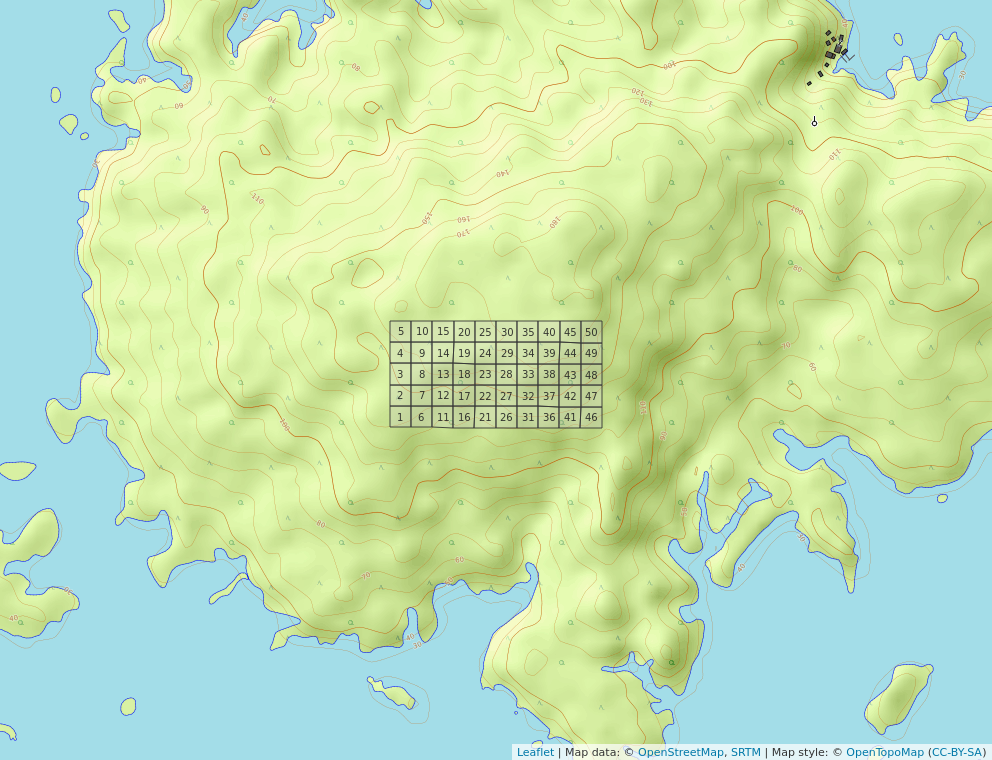
\includegraphics[width=0.50000\textwidth]{mapa_cuadros.png}
\caption{Parcela permanente de 50-ha dela isla Barro Colorado, lago
Gatún, Panamá \label{fig:mapa_cuadros_bci}}
\end{figure}

Materiales y Métodos

Se exploraron los datos del censo número 8 disponibles en la página web
del censo (Hubbell et al., 2021), organizados en dos matrices: la matriz
de comunidad, la cual recopila la información referente a las especies
de la parcela permanente de 50-ha, y la matriz ambiental, que contiene
la información referente a las variables de suelo, geomorfológicas,
litológicas y de tipo de habitat. Los análisis, tablas, figuras y
gráficos se realizaron con los scripts de análisis de José R. Martínez
(Batlle, 2020) y con ayuda de los paquetes de R para análisis
estadísticos y ecológicos (R Core Team, 2019), cabe destacar los
paquetes \texttt{vegan} (Oksanen et al., 2019), \texttt{tidyverse}
(Wickham, 2017), \texttt{sf} (Pebesma, 2018), \texttt{mapview}
(Appelhans, Detsch, Reudenbach, \& Woellauer, 2019) y \texttt{leaflet}
(Cheng, Karambelkar, \& Xie, 2018) que fueron los más utilizados.

A. Medición de asociación

Para calcular la asociación entre especies, se utilizó distancia
chi-cuadrado y la distancia de Jacard: la primera es la distancia
euclidiana calculada sobre los datos transformados, la cual es apropiada
tanto para los datos cuantitativos como para los de presencia-ausencia;
y la segunda, la distancia de Jaccard (** D J \textbf{) se puede
expresar como ``la proporción de especies no compartidas''. La distancia
de Jaccard es el complemento a 1 de la similaridad de Jaccard (} S J
\textbf{), es decir , } D J = 1-S J \textbf{, de esta manera para
obtener la similaridad, sólo hay que restarle el valor de distancia a 1
(} S J = 1-D J **). Se puede usar para evaluar la distancia entre
especies, usando como fuente la matriz de comunidad transpuesta
convertida a binaria (presencia / ausencia) (Batlle, 2020).

El coeficiente de correlación de Pearson tiene como objetivo medir la
fuerza o grado de asociación entre dos variables aleatorias
cuantitativas que poseen una distribución normal bivariada conjunta.
Alternativamente cuando este no cumple con los supuestos se utiliza
coeficiente de correlación no paramétrico de Spearman, se define como el
coeficiente de correlación lineal entre los rangos Ri(x) y Ri(y)
{[}Restrepo (n.d.)\}.

B. Agrupamiento (cluster analysis)

El método con la correlación cofenética se utilizó para escoger los
métodos de agrupamiento, bajo el criterio de que el agrupamiento con la
correlación cofenética más alta puede considerarse como el que produce
el modelo de agrupación que retiene la mayor parte de la información
contenida en la matriz de disimilitud, no obstante, esto no significa
necesariamente que este método sea el más adecuado para el objetivo del
investigador. Luego para escoger una cantidad óptima de clusters para
cada agrupamiento se utilizó la anchura de la silueta, ésta es una
medida del grado de pertenencia de un objeto a su clúster, basada en la
disimilitud media entre este objeto y del clúster al que pertenece,
comparada con la misma medida del clúster más próximo (Borcard, n.d.).

Los métodos aglomerativos utilizados para constatar y evaluar los grupos
que hacían sentido para las mirtáceas de este estudio son desarrollados
a continuación:

-El método aglomerativo por enlace simple (single), conocido como la
clasificación por vecinos más cercanos, aglomera objetos en función de
sus disimilitudes más cortas entre pares: la fusión de un objeto con un
grupo en un nivel de disimilitud determinado sólo requiere que un objeto
de cada grupos que van a aglomerarse esté vinculado al otro en ese
nivel. En consecuencia, el dendrograma resultante de una aglomeración de
enlace simple suele mostrar encadenamiento de objetos. La lista de las
primeras conexiones que hacen a un objeto miembro de un clúster, o que
permite la fusión de dos clústeres, se denomina cadena de conexiones
primarias; esta cadena forma el árbol de expansión mínima (MST).

-El método aglomerativo por enlace completo (complete), conocido como la
clasificación del vecino más lejano, permite que un objeto se agrupe con
otro grupo sólo en la disimilitud correspondiente a la del par de
objetos más distante; de esta manera con mayor motivo, todos los
miembros de los dos grupos están vinculados. Un grupo admite un nuevo
miembro sólo a una disimilitud correspondiente al objeto más lejano del
grupo. De ello se deduce que cuánto más grande es un grupo, más difícil
es aglomerarse con él. La vinculación completa resulta en muchos grupos
pequeños separados que se aglomeran a grandes distancias, por lo que
este método es interesante para buscar e identificar discontinuidades en
los datos.

-El método de grupos de pares no ponderados con media aritmética (UPGMA,
por sus siglas en inglés) es el más conocido de la familia métodos
aglomerativos por enlace promedio, éstos se basan en las disimilitudes
medias entre los objetos o en los centroides de los grupos. El método
UPGMA permite que un objeto se una a un grupo en la media de las
disimilitudes entre este objeto y todos los miembros del grupo. Cuando
dos grupos se unen, lo hacen a la media de las disimilitudes entre todos
los miembros de un grupo y todos los miembros del otro.

-El método de agrupación de varianza mínima de Ward se basa en el
criterio del modelo lineal de mínimos cuadrados. Su objetivo es definir
los grupos de tal manera que la suma de cuadrados dentro del grupo (es
decir, el error cuadrado del ANOVA) se minimiza. La suma de errores al
cuadrado dentro del grupo puede calcularse como la suma de las
distancias al cuadrado entre los miembros de un grupo dividido por el
número de objetos. Este método fue seleccionado porque hace más sentido
ecológico para el estudio(Borcard, n.d.).

El remuestreo \emph{bootstrap} consiste en muestrear aleatoriamente
subconjuntos de los datos y calcular la agrupación en estos
subconjuntos. Luego de repetir este proceso un gran número de veces, se
cuenta la proporción de los resultados de clustering replicados en los
que aparece un cluster determinado. Esta proporción se denomina
probabilidad \emph{bootstrap} (BP) del cluster. El remuestreo
\emph{bootstrap} multiescalar utiliza muestras \emph{bootstrap} de
varios tamaños diferentes para estimar el valor p de cada conglomerado.
Esta mejora produce valores p ``aproximadamente insesgados'' (AU)
(Borcard, n.d.).

Las pruebas que se utilizaron para hacer el correlograma entre los
grupos Ward y las variables ambientales fueron ANOVA, que evalúa
homogeneidad de medias, y Kruskal-Wallis, que evalúa la homogeneidad de
medianas; los cuales hacen sentido para agrupamientos de 3 grupos o
más(Batlle, 2020).

El análisis de especies indicadoras de los grupos Ward se hizo mediante
el índice IndVal, el cual se calcula como el producto de la
especificidad de una especie para el grupo objetivo por su fidelidad al
grupo objetivo. La especificidad se define por la abundancia media de la
especie dentro del grupo objetivo comparada con su abundancia media en
todos los grupos; la fidelidad es la proporción de sitios del grupo
objetivo en el que está presente la especie. Y el análisis de especies
con preferencia por hábitat se realizó mediante el coeficiente de
correlación biserial puntual(Borcard, n.d.).

C. Diversidad Para medir la diversidad alpha se utilizaron los índices
de diversidad, descritos a continuación: -La equidad de Pielou
(denominada también equidad de Shannon) equivale a \emph{J=H1/H0}. -Los
tres primeros números de diversidad de Hill : \emph{N0=q} (la riqueza de
especies), \emph{N1=exp(H)}(número de especies abundantes), y
\emph{N1=1/λ} (inverso de Simpson). -Los ratios de Hill: \emph{E1=N1/N0}
(versión de la \textbf{equidad de Shannon}) y \emph{E2=N2/N0} (versión
de la \textbf{equidad de Simpson}).

Basándonos en los supuestos de Whittaker, que dicen que la diversidad
beta es la variación espacial de la diversidad entre sitios, medimos la
diversidad beta en función de las especies y sitios que contribuían a
ésta con la función \texttt{determinar\_contrib\_local\_y\_especie} de R
del script fuente (Batlle, 2020).

E. Ecología espacial Para medir los patrones de ecología espacial de las
especies y las variables ambientales se utilizaron los modelos de
distribución de especies. Primero se aplicó la prueba I de Moran que
está contenida en la función \texttt{calcular\_autocorrelacion}. Luego,
se aplicó la prueba Yo de Moran a las variables ambientales y las
abundancias de especies transformadas sin tendencia, lo que resultó en
unos clusters lisa que mostraron los patrones significativos de los que
se pueden inferir las dependencias inducidas.

\section{Resultados}\label{resultados}

La familia Myrtaceae está presente en la parcela permanente de 50-ha de
BCI con una abundancia de 5,579 individuos pertenecientes a 7 especies,
de las cuales las más abundantes son \emph{Eugenia galalonensis} y
\emph{Eugenia oerstediana}, representadas con 1,975 y 1,838 individuos
cada una, y las especies más raras son \emph{Psidium
friedrichsthalianum} y \emph{Myrcia gatunensis}, con 58 y 56 individuos
respectivamente (ver tabla \ref{tab:abun_sp}).

\begin{longtable}[]{@{}lr@{}}
\caption{\label{tab:abun_sp}Abundancia por especie de la familia
Myrtaceae}\tabularnewline
\toprule
Latin & n\tabularnewline
\midrule
\endfirsthead
\toprule
Latin & n\tabularnewline
\midrule
\endhead
Eugenia galalonensis & 1975\tabularnewline
Eugenia oerstediana & 1838\tabularnewline
Eugenia coloradoensis & 609\tabularnewline
Chamguava schippii & 541\tabularnewline
Eugenia nesiotica & 502\tabularnewline
Psidium friedrichsthalianum & 58\tabularnewline
Myrcia gatunensis & 56\tabularnewline
\bottomrule
\end{longtable}

\begin{figure}
\centering
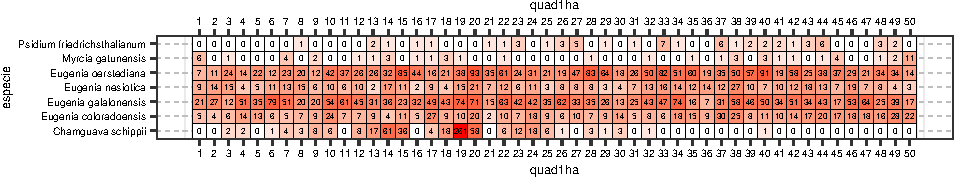
\includegraphics{manuscrito_files/figure-latex/unnamed-chunk-3-1.pdf}
\caption{\label{fig:abun_sp_q}Abundancia de especies por quadrat}
\end{figure}

La distancia de chi-cuadradado y la distancia de Jacard infieren que las
especies del genéro \emph{Eugenia} presentan un patrón de dependencia
(\emph{E. oerstediana}, \emph{E. galalonensis}, \emph{E. nesiotica} y
\emph{E. coloradoensis}), debido a que tienen distancias euclideas muy
pequeñas, es decir, altos grados de asociación; y las especies
\emph{Psidium friedrichsthalianum}, \emph{Myrcia gatunensis} y
\emph{Changuava schippii} presentan un posible patrón independiente, no
parecen asociarse con otras (ver \ref{fig:matriz_Jacard}). El índice de
correlación de Pearson y de Spearman infieren que estos patrones pueden
estar produciéndose debido a la disponibilidad de \emph{Al, P} y escasez
de \emph{Ca}, y a la presencia de los atributos del terreno
geomorfología de llanura, elevación media y a una relación negativa con
la heterogeneidad ambiental, geomorfología de vertiente, geomorfología
de vaguada y pendiente media (ver correlogramas \ref{fig:matriz_pearson}
y \ref{fig:matriz_spearman}).

\begin{figure}
\centering
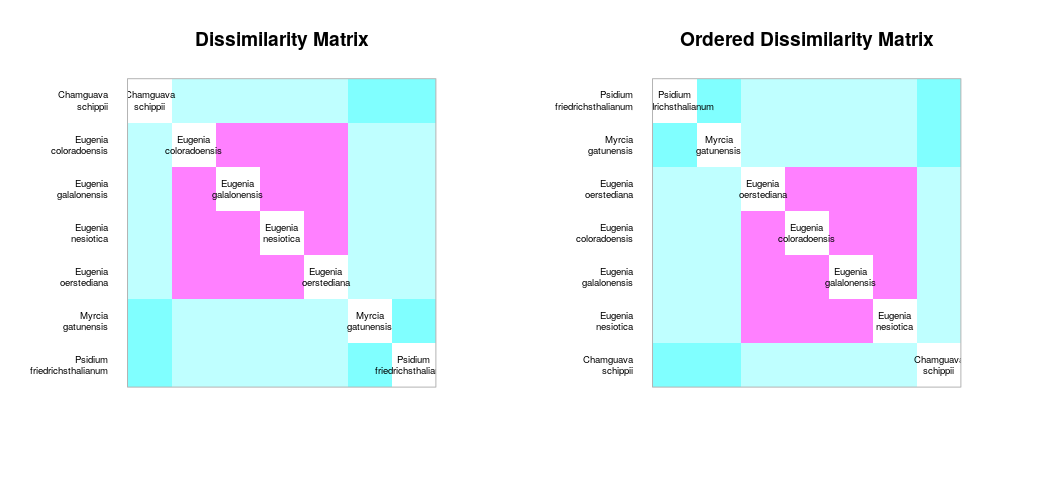
\includegraphics{Disimilaridad_.png}
\caption{Matriz de disimilaridad de Jacard \label{fig:matriz_Jacard}}
\end{figure}

\begin{figure}
\centering
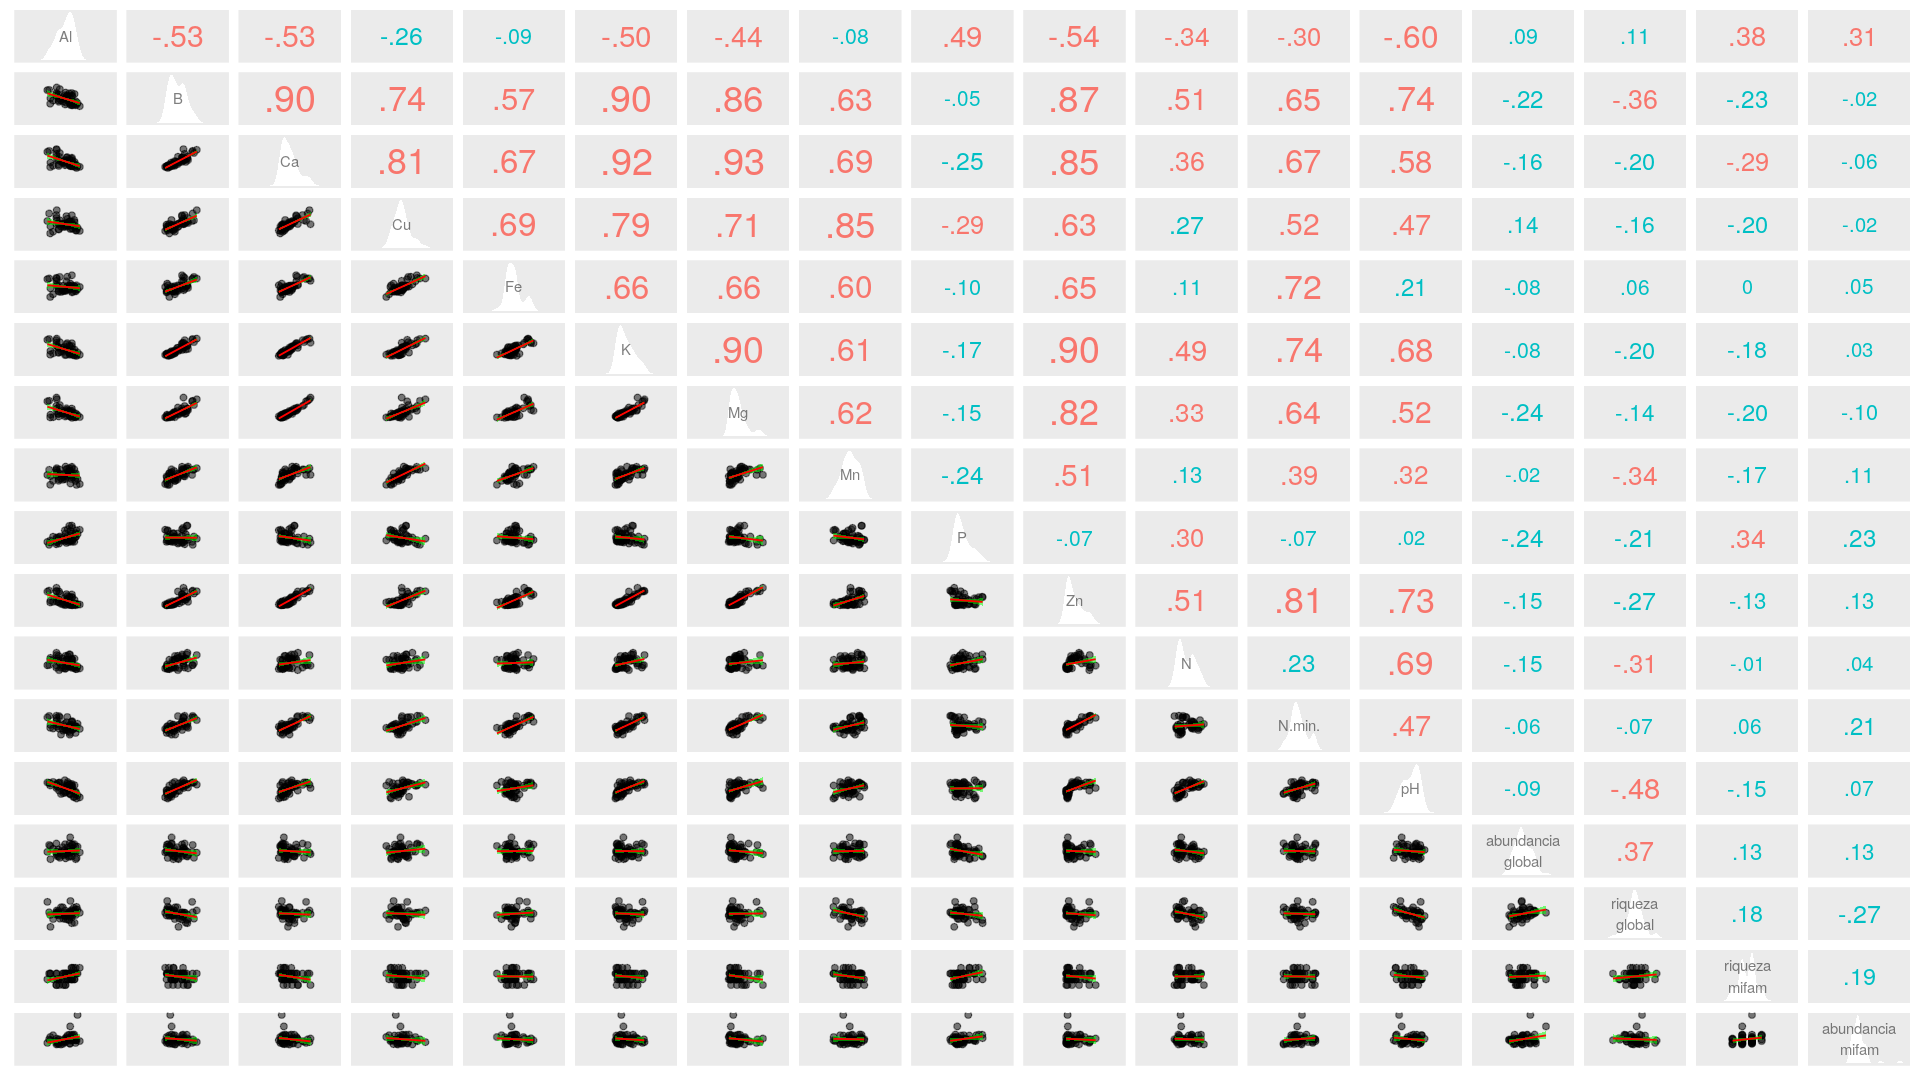
\includegraphics{matriz_correlacion_suelo_abun_riq_spearman.png}
\caption{Matriz de correlación, índice de Spearman
\label{fig:matriz_spearman}}
\end{figure}

El método de agrupamiento Ward de varianza mínima en comparación con el
mapa de calor sugiere que las mirtáceas de la parcela permanente de
50-ha de BCI se distribuyen en 4 grupos, de 2, 13, 15 y 20 sitios,
respectivamente (ver mapa \ref{fig:mapa_ward}). Los métodos de
agrupamiento aglomerativos por enlace simple, por enlace completo y por
enlace promedio (grupos de pares no ponderados con media aritmética,
UPGMA por sus siglas en inglés) destacan la singularidad de este grupo
formado por dos sitios (14 y 19), en suma, el muestreo de
\emph{bootstrap} multiescalar respalda este grupo con un probabilidad de
\emph{bootstrap} (BP) de 76 \% y probabilidad de valores aproximadamente
insesgados (AU) de 99 \%, de que se un grupo real (ver dendrograma
\ref {fig:*bootstrap*_multiescalar}). No hay patrones consistentes con
alguna variable ambiental o atributo, aunque las mirtáceas tienen claras
preferencias por el conjunto de variables (\emph{Al, Fe, Mn, N. min.},
etc.) y atributos del terreno (curvatura perfil media, curvatura
tangencial media, elevación media, etc.) (ver correlograma
\ref{fig:ward_con_variables}).

\begin{figure}
\centering
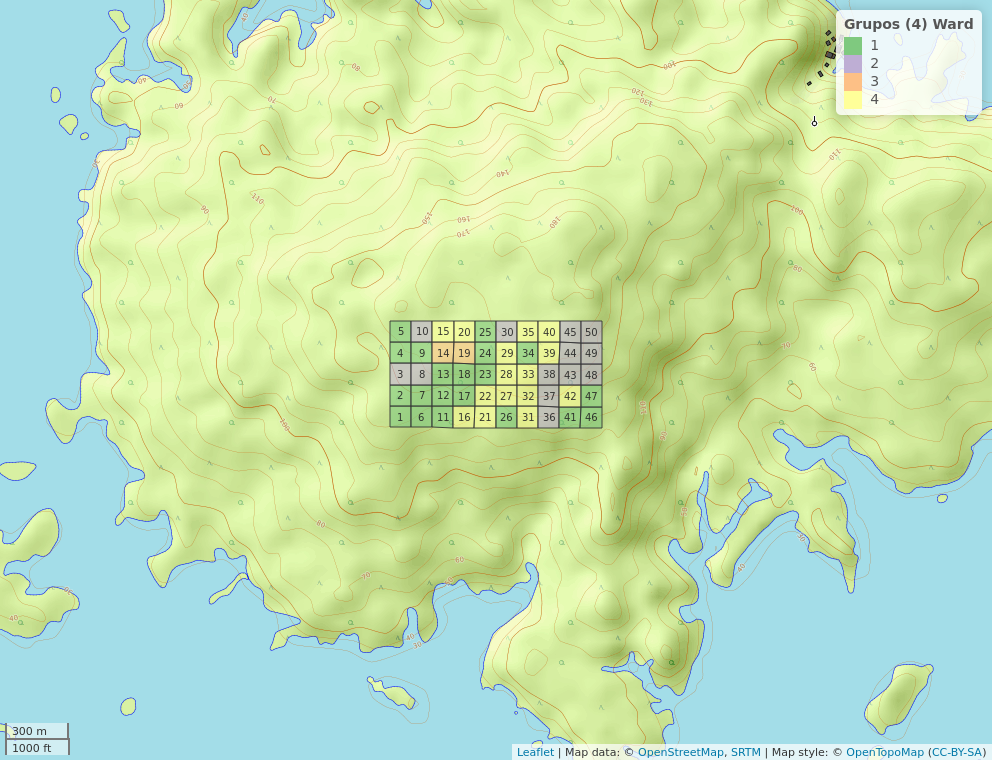
\includegraphics[width=0.50000\textwidth]{mapa_ward_k4.png}
\caption{Agrupamiento por el método Ward de varianza mínima de las
mirtáceas \label{fig:mapa_ward}}
\end{figure}

\begin{figure}
\centering
\includegraphics{*bootstrap*_Ward.png}
\caption{Dendrograma, agrupamiento Ward con los porcentajes del
remuestreo de \emph{bootstrap} multiescalar
\label{fig:*bootstrap*_multiescalar}}
\end{figure}

\begin{figure}
\centering
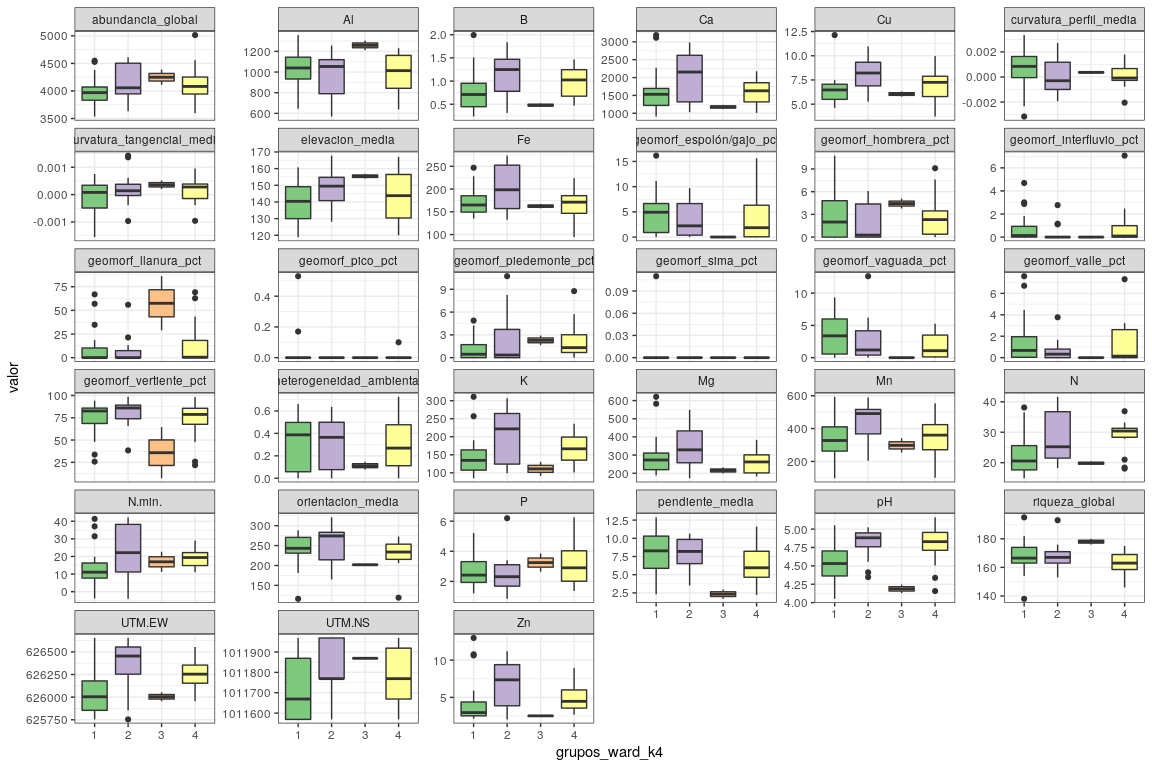
\includegraphics{correlograma_wardyvariablesambientales.png}
\caption{Correlograma grupos Ward con variables ambientales y atributos
\label{fig:ward_con_variables}}
\end{figure}

Para este agrupamiento, el análisis de especies indicadoras mediante
IndVal para una significancia menor de 0.005, propuso como especie
asociada como indicadora del grupo 3 a \emph{Chamguava schippii}, para
el conjunto de grupos 1+2 \emph{Eugenia coloradoensis} y para el
conjunto de grupos 3+4 \emph{Eugenia oerstediana}; y el análisis de
especies con preferencia por hábitat mediante el coeficiente de
correlación biserial puntual para una significancia menor de 0.005,
sugirió que \emph{Eugenia coloradoensis} tiene preferencia por el grupo
2, \emph{Chamguava schippii} por el grupo 3 y \emph{Eugenia oerstediana}
por el grupo 4.

Según los análisis de estimación de riqueza (Homogeneous model,
Homogeneous, los Chao y los Jacknife), la completitud de muestra se
alcanzó al 100\% para las mirtáceas de este ámbito geográfico por lo que
no sería necesario aumentar el esfuerzo de muestreo ya que no se espera
encontrar otras especies en BCI. La diversidad alpha para los grupos
Ward, los cuatro presentaban la riqueza máxima (7 especies) con
diferentes abundancias (1882, 1205, 553 y 1939, respectivamente). Para
los grupos Ward, la riqueza máxima fue estimada y observada, por lo que
también se alcanzó la completitud de muestra al 100\% y al 98\% para el
grupo 3 (grupo con la menor abundancia), y no será necesario aumentar
los esfuerzos de muestreo.

La riqueza (N0), E2 y N2 de Hill sugieren que la diversidad de mirtáceas
presenta una correlación positiva importante con \emph{Al, P, Ca y Fe},
en suma la equidad de Pielou (J), los ratios de Hill (E1 y E2) y N2
infieren una correlación positiva notable con la presencia de la
geomorfología de pendiente media.

\emph{Changuava schipii} y \emph{Eugenia oerstediana} son las especies
que hacen contribución a la diversidad beta, éstas están bien
representadas (la primera con gran dominancia) en los sitios 14 y 19
(grupo 3 Ward) que hacen contribución a la diversidad beta, el 14 es uno
de los cinco sitios que poseen la riqueza máxima (los demás sitios son
13, 17, 22 y 40). Este patrón puede estar relacionado con las
preferencias de este grupo.

La prueba I de Moran sugiere que las mirtáceas de esta localización
presentan patrones aglomerados al menos con la vecindad de primer orden
que implica hasta 50 sitios, con excepción de \emph{M. gatunensis} que
muestra un patrón espacial aleatorio. Cabe destacar que para \emph{C.
schipii} existe una autocorrelación espacial en términos positivos
también para los vecinos de segundo orden y en términos negativos del
cuarto al sexto orden; para \emph{E. nesiotica} y \emph{E. oerstediana}
una autocorrelacion negativa con vecinos de tercer a cuarto orden y de
cuarto a quinto orden, respectivamente, es decir, su abundancia
disminuye en esas vecindades cuando aumenta en la de primer orden y
viceversa. El modelo de abundancia de especies muestra que el 56\% de la
comunidad presenta mayores valores de equidad (log normal 10\% y null
46\%).

La autocorrelación mediante la prueba de Mantel muestra que hay una
correlación espacial inducida por alguna variable en términos positivos
para el primer orden y en términos negativos para el tercer y sexto
orden (hasta 500 metros). La prueba Yo de Moran evidencia que \emph{C.
schipii} muestra un posible patrón de correlación inversa con el
\emph{B, Ca, Zn, N y pH}; para \emph{E. coloradoensis} infiere un patrón
en términos positivos con \emph{Ca} y \emph{N. min.} y de igual manera
para \emph{E. galalonensis} con la geomorfología de vaguada pct y
pendiente media.

\section{Discusión}\label{discusiuxf3n}

La comunidad de mirtáceas de la parcela permante de BCI posee una
riqueza de 7 especies con una abundancia de 5579 individuos, la mayor
abundancia se registró para las especies \emph{E. galalonensis}
(35.40\%) y \emph{E. oerstediana} (32.94\%) y la menor abundancia para
las especies \emph{P. friedrichsthalianum} (1.04\%) y \emph{M.
gatunensis} (1.004\%). En cada quadrat de la parcela BCI podemos
encontrar un mínimo de 58 y un máximo de 399 mirtáceas para un promedio
de 112 individuos por quadrat.

El 57\% de la riqueza, las especies del género \emph{Eugenia},
presentaron altos grados de asociación entre ellas, por lo que supone un
patrón de dependencia, a diferencia de las especies \emph{P.
friedriechsthalianum}, \emph{M. gatunensis} y \emph{C. schipii}
mostraron un posible patrón independiente, por lo que supone que se
presentan aleatoriamente en la muestra sin asociarse a las otras
especies.

Las mirtáceas de esta muestra, según el método Ward, se dividen en 4
grupos, cada uno con 2, 13, 15 y 20 sitios respectivamente; el grupo con
2 sitios es respaldado por los métodos de agrupamiento aglomerativo y el
\emph{bootstrap} multiescalar (BP de 76\% y un AU de 99\%) esto infiere
que es un grupo natural y real dentro de la localidad. Este agrupamiento
no se relaciona específicamente con alguna variable sino por la
preferencia de un conjunto de éstas, como lo son \emph{Al} y \emph{Fe}.

Según el análisis de especies indicadoras (IndVal), las especies
asociadas como diagnósticas para el agrupamiento Ward, fueron \emph{C.
schipii} para el grupo 3, \emph{E. coloradoensis} para el conjunto 1+2 y
\emph{E. oerstediana} para el grupo 3+4, esto puede ser debido a sus
altas abundancias presentes en estos grupos.

Los estimadores de riqueza demostraron que la completitud de muestra
para las mirtáceas en estudio fue alcanzda 100\%, lo mismo para los
grupos Ward, por lo que inferimos que el esfuerzo de muestreo surtió las
necesidas de lugar y no se espera encontrar más especies de en de esta
familia en BCI.

Los equidad de Pielou, los números de Hill destacan que la diversidad de
mirtáceas posee una correlación positiva con \emph{Al, P, Ca, Fe} y la
geomorfología de pendiente media.

Las especies que hacen contribución a la diversidad beta son \emph{C.
schipii} y \emph{E. oerstediana}, y los sitios que hacen contribución a
esta diversidad son el grupo 14 y 19, coincidencialmente un grupo Ward
que posee altas abundancias de las especies antes mencionadas, por lo
que este grupo guarda una estrecha relación con la presencia de estas
especies.

Las mirtáceas de esta localidad, según el I de Moran, presentan patrones
aglomerados para vecinos de primer orden que implican hasta 50 sitios,
con excepción de \emph{M. gatunencis}, que como había mencionado antes,
presentó un patrón aleatorio; en el caso de \emph{C. schipii}, presenta
patrón más aglomerado que las demás debido a que presenta una
correlación positiva también con los vecinos de segundo orden y en
términos negativos con los vecinos del cuarto al sexto orden, es decir
que aumenta o disminuye de forma inversa en estos lugares en relación
con el primer y segundo orden.

El modelo de abundancia de especies muestra que el 56\% de la comunidad
presenta mayores valores de equidad (log normal 10\% y null 46\%),
parece una cifra razonable debido a que el 48\% de los quadrats poseen
valores 7 y 6 de riqueza, lo que infiere que los modelos de distribución
de especies (SDM) parecen estar prediciendo bien la ocurrencia de dichas
especies.

\section{Agradecimientos}\label{agradecimientos}

\section{Información de soporte}\label{informaciuxf3n-de-soporte}

\ldots

\section{\texorpdfstring{\emph{Script}
reproducible}{Script reproducible}}\label{script-reproducible}

\ldots

\section*{Referencias}\label{referencias}
\addcontentsline{toc}{section}{Referencias}

\hypertarget{refs}{}
\hypertarget{ref-mapview}{}
Appelhans, T., Detsch, F., Reudenbach, C., \& Woellauer, S. (2019).
\emph{Mapview: Interactive viewing of spatial data in r}. Retrieved from
\url{https://CRAN.R-project.org/package=mapview}

\hypertarget{ref-jose_ramon_martinez_batlle_2020_4402362}{}
Batlle, J. R. M. (2020). biogeografia-master/scripts-de-analisis-BCI:
Long coding sessions (Version v0.0.0.9000).
\url{https://doi.org/10.5281/zenodo.4402362}

\hypertarget{ref-borcard2018numerical}{}
Borcard, F. ~. ois y L., Daniel y Gillet. (n.d.). \emph{Ecología
numérica con r} (Springer, Ed.).

\hypertarget{ref-leaflet}{}
Cheng, J., Karambelkar, B., \& Xie, Y. (2018). \emph{Leaflet: Create
interactive web maps with the javascript 'leaflet' library}. Retrieved
from \url{https://CRAN.R-project.org/package=leaflet}

\hypertarget{ref-webcenso}{}
Hubbell, S., Condit, R., \& Foster, R. (2021). Forest Census Plot on
Barro Colorado Island. Retrieved May 5, 2021, from
\url{http://ctfs.si.edu/webatlas/datasets/bci/}

\hypertarget{ref-vegan}{}
Oksanen, J., Blanchet, F. G., Friendly, M., Kindt, R., Legendre, P.,
McGlinn, D., \ldots{} Wagner, H. (2019). \emph{Vegan: Community ecology
package}. Retrieved from \url{https://CRAN.R-project.org/package=vegan}

\hypertarget{ref-sf}{}
Pebesma, E. (2018). Simple Features for R: Standardized Support for
Spatial Vector Data. \emph{The R Journal}, \emph{10}(1), 439--446.
\url{https://doi.org/10.32614/RJ-2018-009}

\hypertarget{ref-perez2005metodologia}{}
Pérez, R., Aguilar, S., Condit, R., Foster, R., Hubbell, S., \& Lao, S.
(2005). Metodologia empleada en los censos de la parcela de 50 hectareas
de la isla de barro colorado, panamá. \emph{Centro de Ciencias
Forestales Del Tropico (CTFS) Y Instituto Smithsonian de Investigaciones
Tropicales (STRI)}, 1--24.

\hypertarget{ref-citadeR}{}
R Core Team. (2019). \emph{R: A language and environment for statistical
computing}. Retrieved from \url{https://www.R-project.org/}

\hypertarget{ref-restrepo2007pearson}{}
Restrepo, J. '. n, Luis F y Gonz ~'a lez. (n.d.). De pearson a spearman.
\emph{Revista Colombiana de Ciencias Pecuarias}.

\hypertarget{ref-tidyverse}{}
Wickham, H. (2017). \emph{Tidyverse: Easily install and load the
'tidyverse'}. Retrieved from
\url{https://CRAN.R-project.org/package=tidyverse}

\hypertarget{ref-wilson2010myrtaceae}{}
Wilson, P. G. (2010). Myrtaceae. In \emph{Flowering plants. eudicots}
(pp. 212--271). Springer.




\newpage
\singlespacing 
\end{document}
